\subsection{Imaging systems}\label{subsec:imaging-systems}
\begin{figure}
    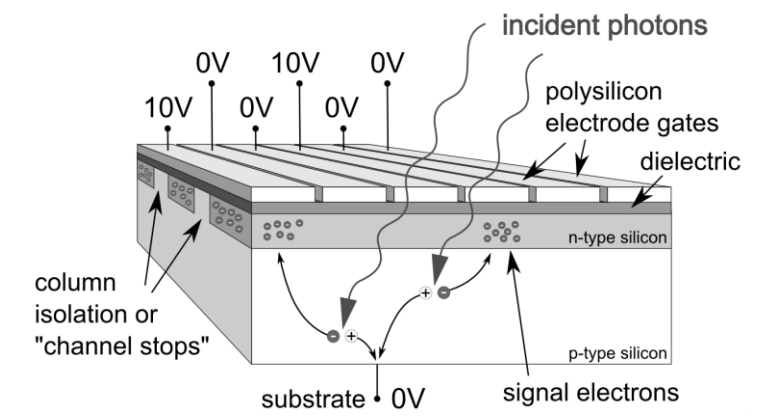
\includegraphics[width=\linewidth,keepaspectratio]{figures/bccd.png}
    \caption{CCD buried channel MOS capacitor\cite{finaltestguideline}}
    \label{fig:mos-cap}
\end{figure}
We begin with a practical discussion of imaging systems. An imaging sensor is a device that converts an optical image into a digital signal.
%
Charge-coupled devices (CCD) and complementary metal-oxide-semiconductor (CMOS) devices are the most common imaging sensors; CCDs have better performance while CMOS devices are newer and less expensive.
%
A third type that's of particular interest to us is the microbolometer, which is used as a sensor in thermal cameras.

CCDs consist of densely packed two-dimensional arrays of buried channel\anote{buriedchannel} MOS capacitors (see figure~\ref{fig:mos-cap}) with an individual MOS capacitor being the fundamental photon detecting element.
%
Individual MOS capacitors are biased by a gate voltage such that a potential well is produced in the n-type silicon (referred to as the n-channel).
%
This potential well acts as a storage system for charge induced by the inner photoelectric effect\anote{innerphotoelectric}.
%
When photons are incident on a MOS capacitor some of the photons are absorbed, some are scattered, and some are transmitted.
%
Those photons that are transmitted interact with electrons in the valence band of the silicon exciting them into the conduction band, and thereby create electron-hole pairs that either diffuse or recombine.
%
For high-quality silicon, the lifetime of such a pair is several milliseconds (before recombination)\cite{scientificccd}.
%
The electrons of the electron-hole pairs that do not recombine diffuse into the potential well, while the holes migrate to the grounded substrate (i.e. out of the sensor).
%
Electrons created in this way are called \textit{photoelectrons}.

CCD arrays consist of two sub-arrays: an image section and a readout section (see figure~\ref{fig:ccd-array}).
%
The image section is arranged with every third stripe of electrode tied electrically to form three sets of equipotentials.
\begin{figure}
    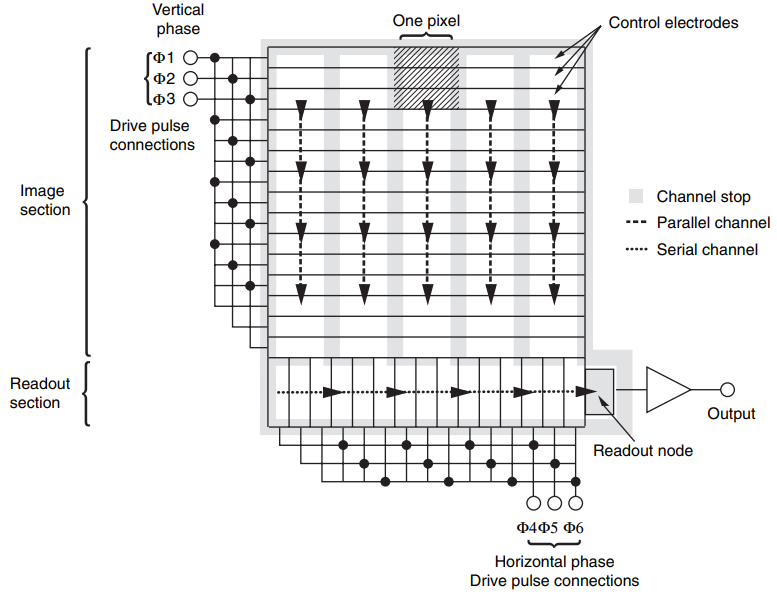
\includegraphics[width=\linewidth,keepaspectratio]{figures/ccd_array.png}
    \caption{CCD array\cite{pawley1995handbook}}
    \label{fig:ccd-array}
\end{figure}
%
In figure~\ref{fig:ccd-array} these equipotentials are labeled $\Phi1, \Phi2, \Phi3$, and taken together constitute a vertical register (VR).
%
They function to move the collected photoelectrons down one electrode line at a time, using charge coupling, while the channel stops function to prevent diffusion of charge across channels.
%
The VR mechanism that shifts collected charge operates as follows:
\begin{enumerate}
    \item Suppose initially there's a collection of photoelectrons on each channel at $\Phi1$ and only $\Phi1$. Note this means $\Phi2, \Phi3$ are at $0$v (again just as in figure ~\ref{fig:mos-cap}).
    \item $\Phi2$ is positively biased to $10$V. This diffuses the collection of charge under both $\Phi1$ and $\Phi2$.
    \item $\Phi1$ is set to $0$v. This concentrates the collection of charge under $\Phi2$.
    \item The same is repeated with $\Phi2, \Phi3$ and $\Phi3, \Phi1$.
    \item The entire process repeats thereby shifting the charge three lines (or one pixel row) at a time.
\end{enumerate}
At the bottom of the image section $\Phi3$ transfers all signal charges to the horizontal register (HR) which functions much like the VR except faster: the HR must transfer every line of pixels independently of all other lines to the read-out node.
%
An obvious challenge faced by this system is how to prevent errant charge from accumulating out of sync with the shift process i.e. how to prevent new photoelectrons from being produced at intermediate lines while far lines are being shifted.
%
The solution is to have interstitial dedicated shift channels in between columns of sensors, with the shift channels being masked off from exposure to light.
%
This type of reading is called \textit{interline transfer} because the accumulated charge is first moved one line over, into the shift channels.
%
Naturally interline transfer shrinks photosensitive area by half and despite possible solutions (e.g micro-lenses being used to focus most of the light onto the unmasked sensors) this is one of the drawbacks of CCDs that CMOS imaging systems do not share.

CMOS sensors consist of arrays of photodiodes (see figure~\ref{fig:photodiode.png}).
\begin{figure}
    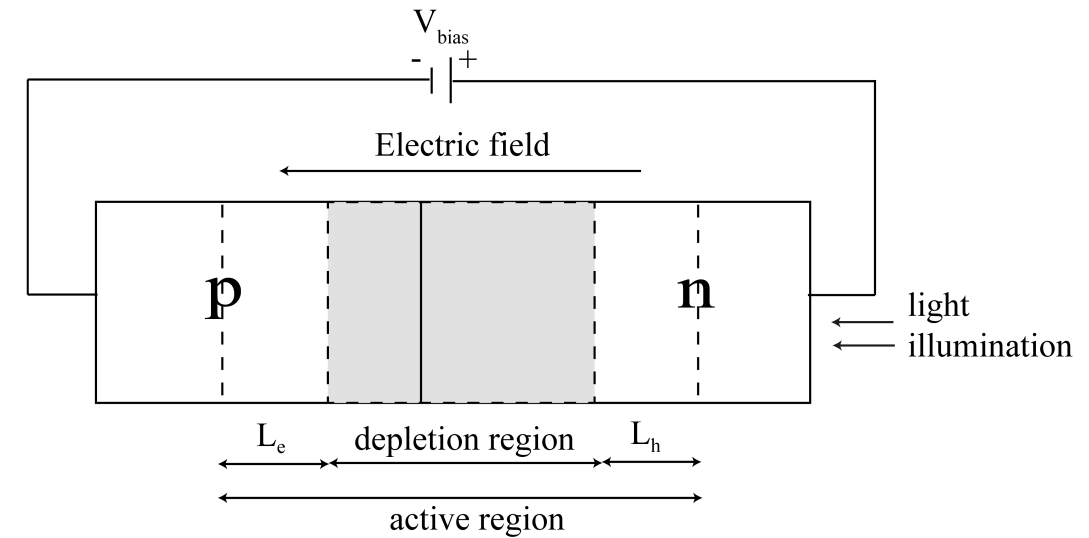
\includegraphics[width=\linewidth,keepaspectratio]{figures/photodiode.png}
    \caption{Photodiode schematic. L\textsubscript{e}, L\textsubscript{h} are electron, hole diffusion lengths respectively\cite{Xu2015FundamentalCO}}
    \label{fig:photodiode.png}
\end{figure}
A photodiode is a p-n junction\anote{pnjunction} operated in reverse bias mode\anote{reversebias}.
%
When a photon of sufficient energy is absorbed by the diode, it creates an electron-hole pair.
%
If the creation event happens within the active region then the hole moves out through the p-type material and the electron moves out through the n-type material.
%
This establishes a \textit{photocurrent} that can be read by a reading circuit (see figure ~\ref{fig:3tpixel}).
\begin{figure}
    \center
    
\includegraphics[width=.5\linewidth,keepaspectratio]{figures/3t_pixel.png}
    \caption{Three transistor "pixel". M\textsubscript{rst} is the reset transistor (enabling the photodiode to dump charge), M\textsubscript{sf} buffers the charge on the photodiode (so that it can be read without loss), and M\textsubscript{sel} enables a whole row of pixels to be read simultaneously (since all pixels in a physical row are tied to the same row line).}
    \label{fig:3tpixel}
\end{figure}
CMOS sensor arrays do not shift the charge from row to row like CCD arrays.
%
In a CMOS sensor array, each pixel contains a transistor M\textsubscript{sel} controlled by the voltage applied across a row (see figure~\ref{fig:cmosarray}).
%
In order to read one row of pixels, a row line is raised high to turn on (close) all the M\textsubscript{sel} transistors in the row.
%
This brings the signals from all the pixels in that row to the shifter register below by way of the column lines.
%
The shift register then outputs the values of the pixels.
%
The high number of transistors needed per pixel in CMOS arrays has only recenty been manageable for semiconductor foundries.
%
This, along with such artifacts as the "rolling shutter" effect produced by rowline reading, are some of the drawbacks of CMOS arrays relative to CCD arrays.
%
Despite this CMOS arrays have become the most common imaging system in consumer goods such as cell phones and digital cameras due to their relatively simple mechanics.
\begin{figure}
    \center
    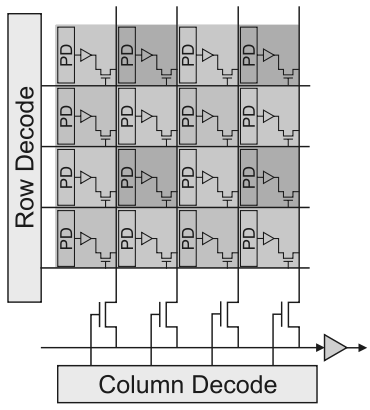
\includegraphics[width=.6\linewidth,keepaspectratio]{figures/cmod.png}
    \caption{CMOS array}
    \label{fig:cmosarray}
\end{figure}

Both CCD arrays and CMOS arrays only capture visible light.
%
A microbolometer, on the other hand, measures the power in the infrared by exposing a thermistor\anote{thermistor} to the incident light.
%
\begin{figure}[b]
    \center
    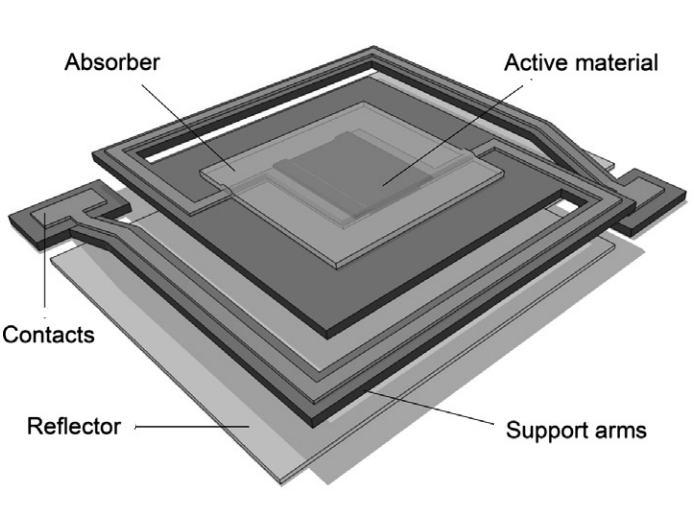
\includegraphics[width=.7\linewidth,keepaspectratio]{figures/microbolometer2.png}
    \caption{Bridge structure of Honeywell microbolometer\cite{KESIM2014245}}
    \label{fig:microbolometer}
\end{figure}
%
Since a thermistor's resistance changes as a function of its temperature, a key issue in the design of a microbolometer is the thermal isolation of the thermistor.
%
With the maturation of micro-machining techniques (such as for MEMS\anote{mems} devices) over the last some years, two level microbolometers consisting of a thermo-sensitive component suspended above (and insulated from) silicon have been built (see figure~\ref{fig:microbolometer}).
%
These pixel packages are evacuated and therefore have good conduction, convection, radiation heat transfer properties.
%
The actual thermo-sensitive component consists of a thermistor, an absorber (which aids in transfer of heat to the thermistor), and a reflector that creates a Fabry–Pérot optical cavity\anote{fabryperot} (typically ${\sim}\lambda/4$\cite{bolometer}) that traps the infrared light.
%
Typical materials for the thermistor are vanadium oxide and amorphous silicon owing to their high temperature coefficients of resistance\cite{bolometer}, which in effect transform small changes in temperature into large changes in resistance.
%
Measurements of the thermistor are performed by a read-out integrated circuit adjacent to the bridge in the silicon substrate.
%
All told microbolometers are designed much differently from either CCD or CMOS arrays.
%
It is as a result of this fact that high-resolution infrared cameras are not available.

Across all of these imaging systems there are ample avenues for the introductions of the kinds of errors that degrade image quality and across all of these imaging systems there are structures that impose limitations on resolving power.
%
With that in mind we now proceed to formalizing the problem of super-resolution.

\subsection{Mathematical notation}\label{subsec:notation}
Upper case plain latin $X, Y$ each denote channel $\times$ row $\times$ column \textit{tensors}\anote{tensor} representing LR and HR images respectively, with $(0, 0,0)$ corresponding to the top left corner of the first channel of image.
%
Often for the sake of simplicity we consider greyscale images, in which case we omit the channel dimension.
%
Lower case plain latin $x, y$ denote LR and HR \textit{patches}\anote{patch} respectively.
%
$D, H, F, G$ variously refer to functions that operate on images.
%
Bolded uppercase latin $\bm{X}, \bm{Y}$ are reserved for batches of images, i.e. batch size $\times$ channel $\times$ row $\times$ column tensors with $(0, 0, 0,0)$ corresponding to the top left corner of the first channel of first image in the batch.
%
Bolded lower case denote $\bm{x}, \bm{y}, \bm{z}$ etc. denote conventional column or row vectors.
%
Unless otherwise specified $\left\| \cdot \right\|$ is the $L_2$ norm.

\subsection{Imaging model}\label{subsec:imaging-model}
Figure~\ref{fig:bertrand} shows a conceptual model of the imaging process as carried out by an imaging system.
%
The input to the system is a natural scene that is in effect sampled by the imaging system.
%
In the idealized case the sampling is done at (or above) the Nyquist rate and no aliasing occurs.
%
In practice there is noise and loss introduced at every step of the process: atmospheric turbulence plays a role at large distances, motion produces multiple views of the same scene but also induces blur, imperfections of the lenses further blur the image, and finally down-sampling by the sensor elements into pixels produces aliasing artifacts\anote{ccd}.
%
The noisy, blurry, down-sampled images are then further degraded by sensor noise.
%
Each such image we call an LR sample.
\begin{figure*}
    \centering
    \begin{adjustbox}{width=\textwidth}
        \begin{tikzpicture}[auto]
            \tikzstyle{terminal} = [rectangle, draw, text width=5em, text centered, minimum height=4em]
            \tikzstyle{block} = [rectangle, draw, fill=gray!20, text width=6em, text centered, rounded corners, minimum height=4em]
            \tikzstyle{line} = [draw, -latex']
            \tikzstyle{sum} = [circle, draw]

            \node[inner sep=0pt] (bertrand) {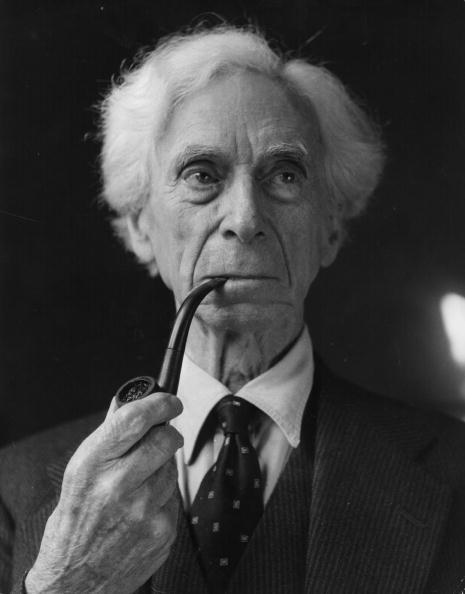
\includegraphics[width=.15\textwidth]{figures/bertrand.png}};
            \node [above = of bertrand] (scene) {Scene};

            \node[sum, right = of bertrand] (sum1) {$+$};
            \node [block, below = of sum1] (atmo-noise) {Atmospheric noise};

            \node [block, right = of sum1] (motion) {Translation, Rotation, Aspect};
            \node [above = of motion] {Motion};

            \node [inner sep=0pt, right = of motion] (motion-output) {};

            \node[inner sep=0pt, below = of motion-output] (bertrand-motion) {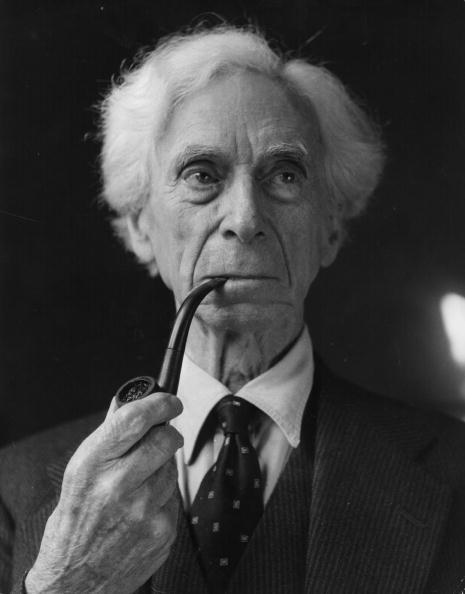
\includegraphics[width=.15\textwidth]{figures/bertrand.png}};
            \node[inner sep=0pt, below = of motion-output, xshift=2mm, yshift=-2mm] {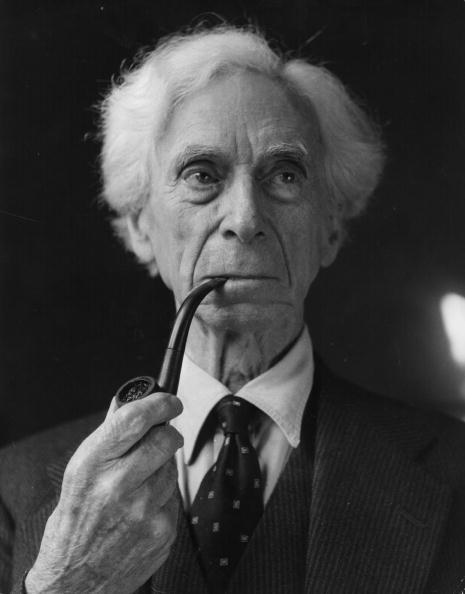
\includegraphics[width=.15\textwidth]{figures/bertrand.png}};
            \node[inner sep=0pt, below = of motion-output, xshift=4mm, yshift=-4mm] {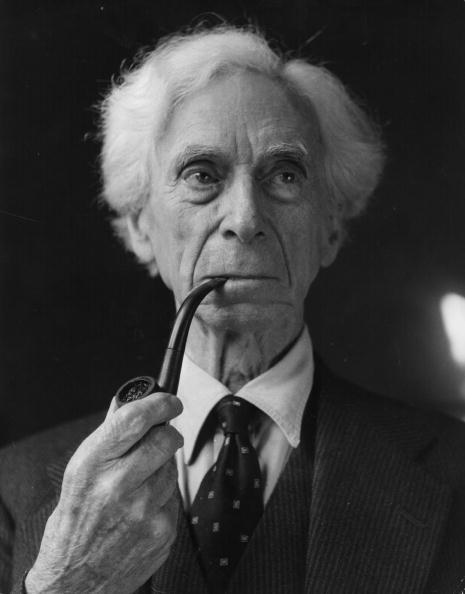
\includegraphics[width=.15\textwidth]{figures/bertrand.png}};
            \node[inner sep=0pt, below = of motion-output, xshift=6mm, yshift=-6mm] {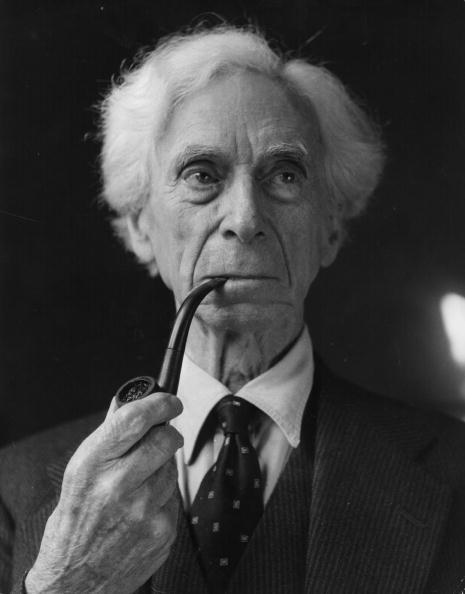
\includegraphics[width=.15\textwidth]{figures/bertrand.png}};

            \node [block, right = of motion-output] (blur) {Optical, Motion};
            \node [above = of blur] {Blur};
            \node [inner sep=0pt, right = of blur] (blur-output) {};

            \node[inner sep=0pt, below = of blur-output] (bertrand-blur) {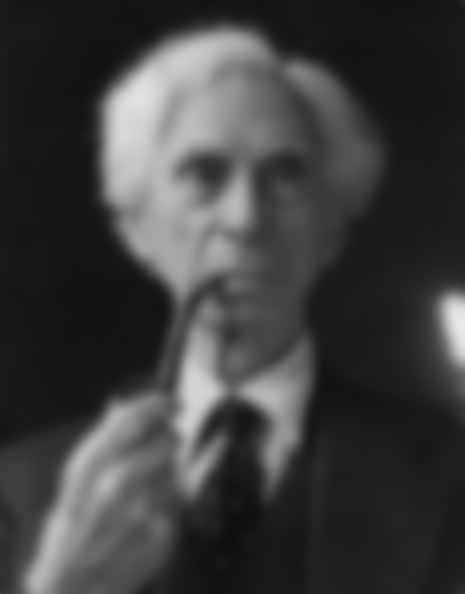
\includegraphics[width=.15\textwidth]{figures/bertrand-blur.png}};
            \node[inner sep=0pt, below = of blur-output, xshift=2mm, yshift=-2mm] {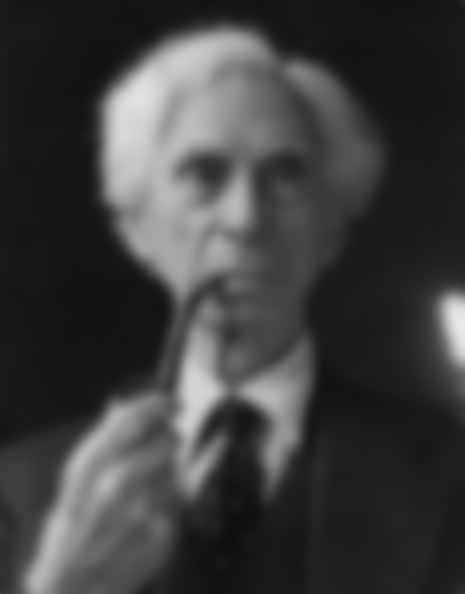
\includegraphics[width=.15\textwidth]{figures/bertrand-blur.png}};
            \node[inner sep=0pt, below = of blur-output, xshift=4mm, yshift=-4mm] {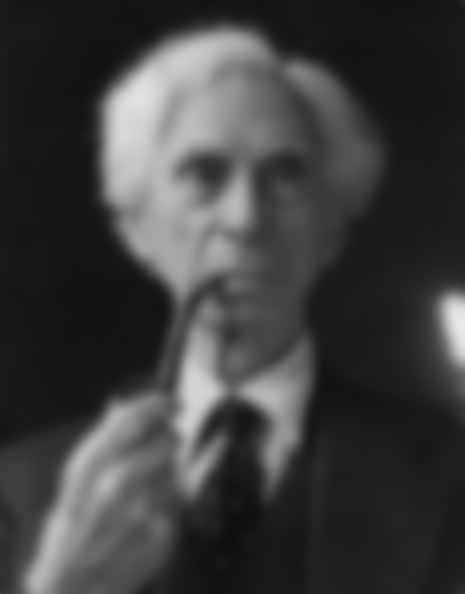
\includegraphics[width=.15\textwidth]{figures/bertrand-blur.png}};
            \node[inner sep=0pt, below = of blur-output, xshift=6mm, yshift=-6mm] {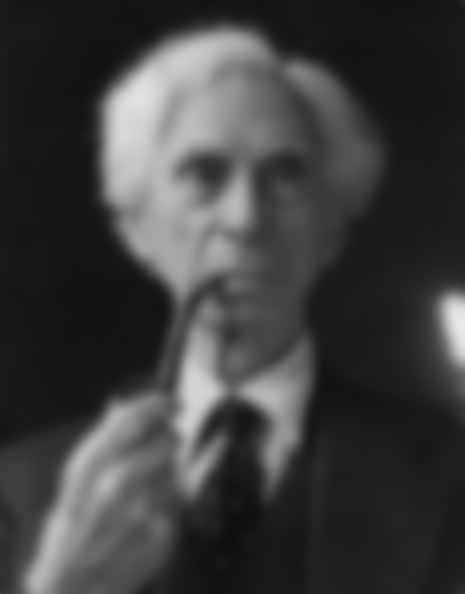
\includegraphics[width=.15\textwidth]{figures/bertrand-blur.png}};

            \node[block, right = of blur-output] (downsample) {Quantization, Pixel-binning};
            \node [above = of downsample] {Down-sampling};

            \node[sum, right = of downsample] (sum2) {$+$};
            \node [block, below = of sum2] (sensor-noise) {Sensor noise};

            \node[inner sep=0pt, right = of sum2] (bertrand-blur-noise) {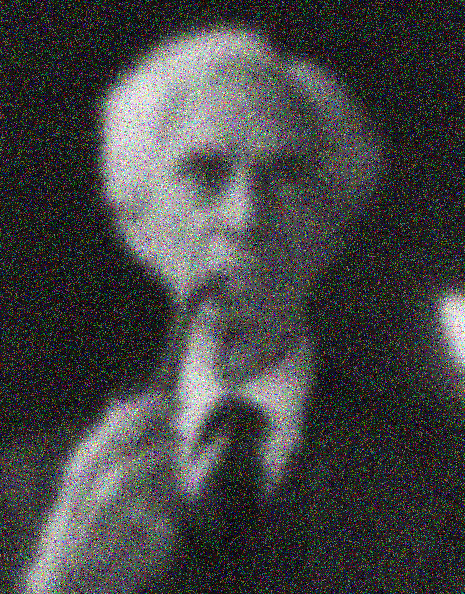
\includegraphics[width=.1\textwidth]{figures/bertrand-blur-noise.png}};
            \node[inner sep=0pt, right = of sum2, xshift=2mm, yshift=-2mm] {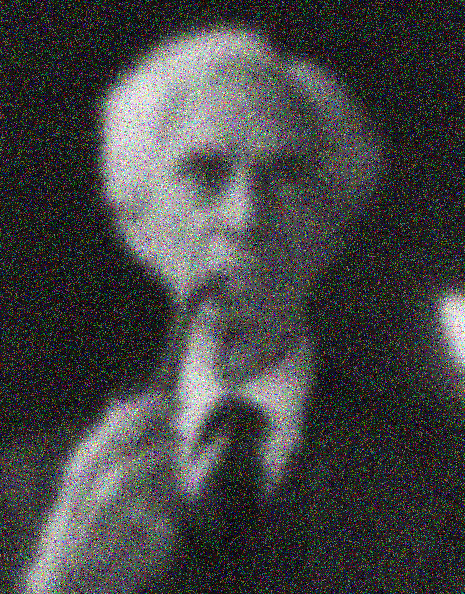
\includegraphics[width=.1\textwidth]{figures/bertrand-blur-noise.png}};
            \node[inner sep=0pt, right = of sum2, xshift=4mm, yshift=-4mm] {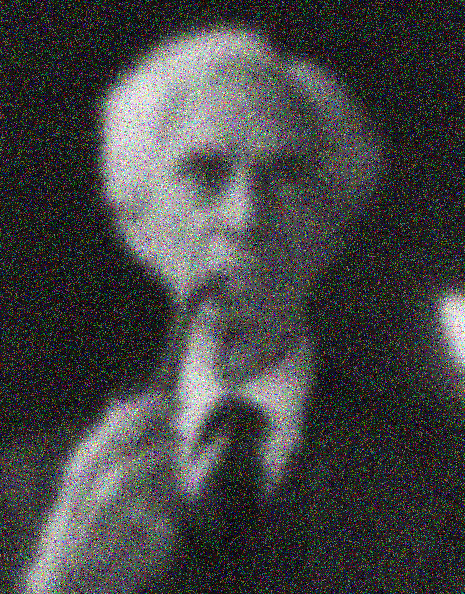
\includegraphics[width=.1\textwidth]{figures/bertrand-blur-noise.png}};
            \node[inner sep=0pt, right = of sum2, xshift=6mm, yshift=-6mm] {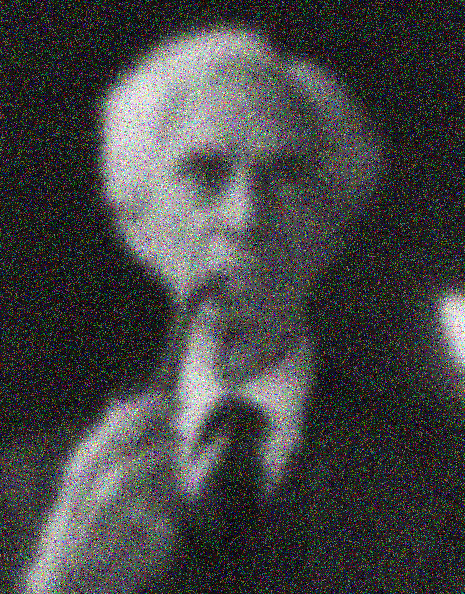
\includegraphics[width=.1\textwidth]{figures/bertrand-blur-noise.png}};
            \node [above = of bertrand-blur-noise, text width=5em] (lr-output) {Low-resolution images};

            \draw[-] (bertrand) edge (sum1);
            \draw[->] (sum1) edge (motion);
            \draw[->] (atmo-noise) edge (sum1);

            \draw[->] (motion) edge (blur);
            \draw[->] (motion-output) edge (bertrand-motion);

            \draw[->] (blur) edge (downsample);
            \draw[->] (blur-output) edge (bertrand-blur);
            \draw[->] (sensor-noise) edge (sum2);
            \draw[-] (downsample) edge (sum2);
            \draw[->] (sum2) edge (bertrand-blur-noise);
        \end{tikzpicture}
    \end{adjustbox}
    \caption{The imaging model illustrating the relationship between a scene and final low-resolution images due to noise, motion, blur, and sampling.}
    \label{fig:bertrand}
\end{figure*}

Let $Y$ denote an idealized HR image of the scene from some fixed vantage point and assume the imaging system collects $K$ LR samples $X_k$ of $Y$.
%
Formally the $X_k$ are related to $Y$ by
\begin{equation}
    X_k = (D \circ H_k \circ A_k) (Y) + \varepsilon_k
    \label{eqn:imagingmodel}
\end{equation}
where for the $k$th sample $A_k$ (of $K$) is the operator representing motion (affine and perspective shift) induced by optical flow\anote{opticalflow}, $H_k$ represents the blur operator, $D$ represents the down-sampling operator (constant in time since it's typically a digital component of the imaging system), and $\varepsilon_k$ represents the composite noise (environment and sensor noise).

We now consider the challenges and nuances of estimating motion and blur.

For a static 3-D scene and an imaging system with 6 degrees of freedom, the optical flow caused by motion is dependent on the geometry of the scene and potentially nonlinear (due to occlusion and motion parallax).
%
This pertains to multiple image registration for MISR where we seek to relate $X_{k+1}$ to $X_k$:
\begin{equation*}
    X_{k+1}(x,y) = X_k(x + v_x(x,y), y + v_y(x,y))
\end{equation*}
%
For small motions we can approximate $X_k$ by its first order Taylor series:
\begin{align}
    X_{k+1}(x,y) &= X_k(x + v_x(x,y), y + v_y(x,y)) \\
    &\approx X_k(x,y) + v_x(x,y)\frac{\partial X_k}{\partial x} + v_y(x,y)\frac{\partial X_k}{\partial y}\label{eqn:opticalflowtaylor}
\end{align}
Evaluating equation~\ref{eqn:opticalflowtaylor} at every pixel gives a set of linear equations that enable us to fit one of the models in table~\ref{table:flow}.
%
We focus on affine flow primarily because it is easy to estimate and secondarily because the composition of multiple affine transformations is an affine transformation (enabling us to register more than 2 images by building up the necessary transformations incrementally).
%
Note that for nonstatic scenes the registration problem becomes "exponentially" more difficult as many more parameters need to be estimated.
%
Furthermore registration and super resolution are not independent since the data being used to estimate the registration transforms is blurry and noisy; to wit perfectly resolved images could be much more effectively registered.

\begin{table*}
    \begin{center}
        \begin{tabular}{ llp{5cm} }
            Flow Type & Model & When Applicable \\
            \\
            \hline
            \\
            Affine & {$\begin{aligned}
                           v_x(x,y) &= p_1 x + p_2 y + p_3 \\
                           v_y(x,y) &= p_4 x + p_5 y + p_6
            \end{aligned}$} & Planar scene with orthographic projection \\
            \\
            Planar Projective & {$\begin{aligned}
                                      v_x(x,y) &= \frac{p_1+p_2 x + p_3 y}{p_7 + p_8 x + p_9 y} - x\\
                                      v_y(x,y) &= \frac{p_4+p_5 x + p_6 y}{p_7 + p_8 x + p_9 y} - y\\
            \end{aligned}$} & Planar scene with full prospective projection \\
            \\
            Quadratic & {$\begin{aligned}
                              v_x(x,y) &= \omega_Z y + \frac{\omega_X xy}{l} - \frac{\omega_Y x^2}{l} - \omega_Y l \\
                              &\approx p_1 y + p_2 xy + p_3 x^2 + p_4 \\
                              v_y(x,y) &= -\omega_Z x - \frac{\omega_Y xy}{l} + \frac{\omega_X y^2}{l} + \omega_X l \\
                              &\approx p_5 y + p_6 xy + p_7 x^2 + p_8 \\
                              &
            \end{aligned}$} & Approximate for prospective projection with only $\omega_X, \omega_Y, \omega_Z$ euler angle rotations ($l$ is focal length) \\
            \\
            Quadratic & {$\begin{aligned}
                              v_x(x,y) &\approx p_1 x + p_2 y + p_3 x^2 + p_4 xy + p_5 \\
                              v_y(x,y) &\approx p_6 x + p_7 y + p_8 y^2 + p_9 xy + p_{10} \\
                              &
            \end{aligned}$} & Approximate for planar scene with full prospective projection\\
            \\
        \end{tabular}
    \end{center}
    \caption{Optical flow models\cite{Trucco:1998:ITC:551277}. Note $x,y$ are pixel coordinates and $p_i$ are parameters that need to be estimated.}
    \label{table:flow}
\end{table*}


In general the optical transfer function (OTF) characterizes the blur of an imaging system\anote{otf}.
%
We factor the OTF into three components:
\begin{equation}
    H(u, v) = H_{\text{diff}}(u,v) H_{\text{abr}}(u,v) H_{\text{int}} (u,v)
\end{equation}
where $u,v$ are horizontal and vertical spatial frequencies respectively (measured in cycles/mm), $H_{\text{diff}}$ is blur due to diffraction, $H_{\text{abr}}$ is blur due to lens aberrations, and $H_{\text{int}}$ is blur due to imaging sensor shape (obtained by taking the Fourier transform of the shape an individual sensor in the imaging array).
%
Blur due to diffraction in most imaging systems is due to diffraction through a circular aperture\cite{goodman2005introduction}:
\begin{equation*}
    H_{\text{diff}}(u,v) =   \begin{cases}
                                 \frac{2}{\pi} \left(\frac{1}{\cos(\tau)} - \tau \sqrt{1-\tau^2}\right) & \text{if } \tau < 0 \\
                                 0 & \text{otherwise}
    \end{cases}
\end{equation*}
where $\tau = \rho/\rho_c$, $\rho=\sqrt{u^2 +v^2}$, $\rho_c = 1/\lambda N$ is the radial cutoff frequency of the aperture, $N$ is the f-number\anote{fnumber} of the optics, and $\lambda$ is the wavelength of light being diffracted.
%
This is in fact the filter that produces the Airy pattern and therefore informs sensor array spacing in order to avoid aliasing.
%
Wavelength independent blurring due to aberrations can be induced by various imperfections in the lenses such as spherical aberration, comatic aberration\anote{coma}, or astigmatism. Furthermore, dispersion\anote{dispersion} blurs particular wavelengths of light. A good model for all of these effects is\cite{10.1117.12.946501}:
\begin{equation*}
    H_{\text{abr}}(u,v) =   \begin{cases}
                                1-\left(\frac{25}{65}\right)^2 \left(1-4\left(\tau - \frac{1}{2}\right)\right)^2& \text{if } \tau < 0 \\
                                0 & \text{otherwise}
    \end{cases}
\end{equation*}
Figure~\ref{fig:mtf} shows an example OTF for an imaging system with a sensor spacing of 0.050 mm and therefore sampling frequency of 20 cycles/mm and $\rho_c = 83.3~\text{cycles}/\text{mm}$ ($F=3$ and $\lambda = 4\mu\text{m}$ i.e. near infrared).
%
Notice that $\rho_c$ is much greater than the Nyquist rate ($\frac{1}{2} \times 20~\text{cycles}/\text{mm} = 10~\text{cycles}/\text{mm}$) and therefore many frequencies that are within the radial cutoff frequency will be aliased.
%
This in particular can be mitigated by effectively increasing sampling rate using MISR.
%
Notice also that like a typical transfer function the OTF is not flat and therefore attenuates high spatial frequencies.
%
Simply applying gain to the image wouldn't solve the attenuation problems because of aliasing, but likewise this can be resolved after the effective sampling rate is increased using MISR.
\begin{figure}
    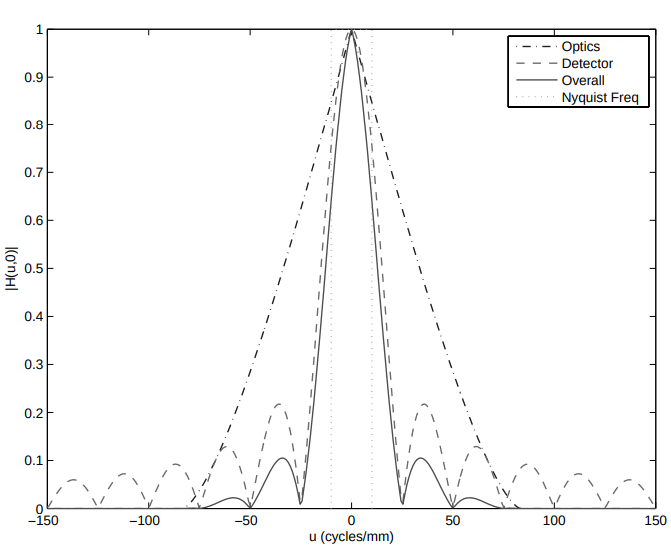
\includegraphics[width=\linewidth,keepaspectratio]{figures/mtf.png}
    \caption{OTF magnitude cross-section for\cite{milanfar2017super}}
    \label{fig:mtf}
\end{figure}

The challenge of super-resolution is to solve the inverse problem of finding $Y$ from one or several $X_k$.
%
In general, since $A_k, H_k, D_k$ are highly degenerate functions, the corresponding inverse problems are ill-posed without regularization and conditioning.
%
The techniques that have been brought to bear on the problem range from interpolation to statistical estimation to example based learning.
